
\appendix
\addcontentsline{toc}{part}{Appendix}
\section*{Appendix} \label{Appendix}
\renewcommand{\thesubsection}{\Alph{subsection}}

\subsection{Commutativity of CZ}

What we want to show here is that if we teleport two photons in parallel, to some modes A and B, and then apply a CZ gate across those modes, this is equivalent to applying a CZ gate \textit{first} and then applying some combination of X and Z gates to teleport our photons. 
\par
For the purposes of keeping this appendix from being longer than need be, we're going to ignore the cases of the Bell Measurement where the identity is applied, it should be fairly trivial to see that $\mathbb{I}(CZ) \equiv (CZ)\mathbb{I}$
\subsubsection{How CZ commutes with X}\label{sec:CZ commute X}
Looking at the second qubit teleportation first, we'll consider the case of the Bell measurement where 'x' = 1, 'z' = 0. Meaning that to teleport $\ket{\phi_2}$ from \ref{fig:QTCZ-2}, we need an X gate applied to the second qubit. This is shown in \ref{fig_APP:X - CZ } where we want to commute the CZ gate from the right to the left.
\\
We first start by writing out what the X gate applied to the second qubit looks like as a matrix. This is:
\begin{align}
    (X \otimes\mathbb{I}) & = 
    \begin{pmatrix}
    0 & 1\\ 
    1 & 0
    \end{pmatrix} 
    \otimes
    \begin{pmatrix}
    1 & 0\\ 
    0 & 1
    \end{pmatrix}
    \\
    & = 
    \begin{pmatrix}
    0 & 0 & 1 & 0\\ 
    0 & 0 & 0 & 1\\
    1 & 0 & 0 & 0\\
    0 & 1 & 0 & 0\\
\end{pmatrix} \label{X tens I}
\end{align}
Which we can confirm is true by applying it to the state $ \ket{2} \equiv \ket{10} \equiv 
\begin{pmatrix}
    0 \\ 
    0\\
    1\\
    0\\
\end{pmatrix}$ and checking if we get the state $\ket{0} \equiv \ket{00} \equiv 
\begin{pmatrix}
    1 \\ 
    0\\
    0\\
    0\\
\end{pmatrix}$
\par
 We also write that the matrix for the 2 qubit CZ gate is:
\begin{equation}
    CZ = 
    \begin{pmatrix}
    1 & 0 & 0 & 0 \\ 
    0 & 1 & 0 & 0 \\
    0 & 0 & 1 & 0 \\
    0 & 0 & 0 & -1\\
    \end{pmatrix}
\end{equation} which we can confirm with the state $\ket{3} \equiv \ket{11}$ which should transform to $-\ket{11}$.


\begin{figure}
    \centering
\tikzset{every picture/.style={line width=0.75pt}} %set default line width to 0.75pt        

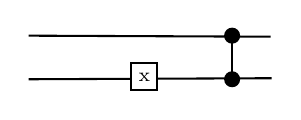
\begin{tikzpicture}[x=0.75pt,y=0.75pt,yscale=-1,xscale=1]
%uncomment if require: \path (0,300); %set diagram left start at 0, and has height of 300

%Straight Lines [id:da732813246379387] 
\draw    (99.83,109.67) -- (216.33,110.17) ;
%Straight Lines [id:da6605550224031504] 
\draw    (99.83,130.67) -- (216.83,130.17) ;
%Straight Lines [id:da2257066549092701] 
\draw    (197.83,109.67) -- (197.83,130.67) ;
\draw [shift={(197.83,130.67)}, rotate = 90] [color={rgb, 255:red, 0; green, 0; blue, 0 }  ][fill={rgb, 255:red, 0; green, 0; blue, 0 }  ][line width=0.75]      (0, 0) circle [x radius= 3.35, y radius= 3.35]   ;
\draw [shift={(197.83,109.67)}, rotate = 90] [color={rgb, 255:red, 0; green, 0; blue, 0 }  ][fill={rgb, 255:red, 0; green, 0; blue, 0 }  ][line width=0.75]      (0, 0) circle [x radius= 3.35, y radius= 3.35]   ;
%Shape: Rectangle [id:dp8096940990542667] 
\draw  [fill={rgb, 255:red, 255; green, 255; blue, 255 }  ,fill opacity=1 ] (149.3,123) -- (161.83,123) -- (161.83,136) -- (149.3,136) -- cycle ;

% Text Node
\draw (151.3,126) node [anchor=north west][inner sep=0.75pt]  [font=\tiny] [align=left] {{\scriptsize x}};


\end{tikzpicture}
    \caption{Caption}
    \label{fig_APP:X - CZ }
\end{figure}

What we want to find then is the combination of X and Z matrices that gives us a matrix equivalent to $CZ(X\otimes\mathbb{I})$. We won't derive it here but we can easily show that $CZ(X\otimes\mathbb{I}) = (X\otimes Z)CZ$:

\begin{align} \label{eqn_APP: CZ commute X}
    CZ(X\otimes\mathbb{I}) & = 
    \begin{pmatrix}
        1 & 0 & 0 & 0 \\
        0 & 1 & 0 & 0 \\
        0 & 0 & 1 & 0 \\
        0 & 0 & 0 & -1 \\
    \end{pmatrix} \cdot
    \begin{pmatrix}
        0 & 0 & 1 & 0 \\
        0 & 0 & 0 & 1 \\
        1 & 0 & 0 & 0 \\
        0 & 1 & 0 & 0 \\
    \end{pmatrix}
    \\ & =
    \begin{pmatrix}
        0 & 0 & 1 & 0 \\
        0 & 0 & 0 & 1 \\
        1 & 0 & 0 & 0 \\
        0 & -1 & 0 & 0 \\
    \end{pmatrix}
    \\ & = 
    \begin{pmatrix}
        0 & 0 & 1 & 0 \\
        0 & 0 & 0 & -1 \\
        1 & 0 & 0 & 0 \\
        0 & -1 & 0 & 0 \\
    \end{pmatrix} \cdot
    \begin{pmatrix}
        1 & 0 & 0 & 0 \\
        0 & 1 & 0 & 0 \\
        0 & 0 & 1 & 0 \\
        0 & 0 & 0 & -1 \\
    \end{pmatrix} 
    \\ & = 
    \left(
    \begin{pmatrix}
        0 & 1 \\
        1 & 0 \\
    \end{pmatrix}
    \otimes
    \begin{pmatrix}
        1 & 0 \\
        0 & -1 \\
    \end{pmatrix}  \right) \cdot 
    \begin{pmatrix}
        1 & 0 & 0 & 0 \\
        0 & 1 & 0 & 0 \\
        0 & 0 & 1 & 0 \\
        0 & 0 & 0 & -1 \\
    \end{pmatrix} 
    \\ & = 
    (X\otimes\mathbb{Z})CZ
\end{align}

\begin{figure}
    \centering
    

\tikzset{every picture/.style={line width=0.75pt}} %set default line width to 0.75pt        

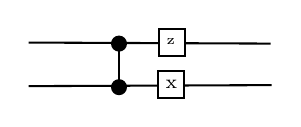
\begin{tikzpicture}[x=0.75pt,y=0.75pt,yscale=-1,xscale=1]
%uncomment if require: \path (0,300); %set diagram left start at 0, and has height of 300

%Straight Lines [id:da732813246379387] 
\draw    (99.83,109.67) -- (216.33,110.17) ;
%Straight Lines [id:da6605550224031504] 
\draw    (99.83,130.67) -- (216.83,130.17) ;
%Straight Lines [id:da2257066549092701] 
\draw    (143.33,110.17) -- (143.33,131.17) ;
\draw [shift={(143.33,131.17)}, rotate = 90] [color={rgb, 255:red, 0; green, 0; blue, 0 }  ][fill={rgb, 255:red, 0; green, 0; blue, 0 }  ][line width=0.75]      (0, 0) circle [x radius= 3.35, y radius= 3.35]   ;
\draw [shift={(143.33,110.17)}, rotate = 90] [color={rgb, 255:red, 0; green, 0; blue, 0 }  ][fill={rgb, 255:red, 0; green, 0; blue, 0 }  ][line width=0.75]      (0, 0) circle [x radius= 3.35, y radius= 3.35]   ;
%Shape: Rectangle [id:dp8096940990542667] 
\draw  [fill={rgb, 255:red, 255; green, 255; blue, 255 }  ,fill opacity=1 ] (162.3,123.5) -- (174.83,123.5) -- (174.83,136.5) -- (162.3,136.5) -- cycle ;
%Shape: Rectangle [id:dp33853823787750703] 
\draw  [fill={rgb, 255:red, 255; green, 255; blue, 255 }  ,fill opacity=1 ] (162.8,103) -- (175.33,103) -- (175.33,116) -- (162.8,116) -- cycle ;

% Text Node
\draw (164.3,126.5) node [anchor=north west][inner sep=0.75pt]  [font=\tiny] [align=left] {{\scriptsize x}};
% Text Node
\draw (164.8,106) node [anchor=north west][inner sep=0.75pt]  [font=\tiny] [align=left] {z};


\end{tikzpicture}

    \caption{Caption}
    \label{fig_APP:CZ-X}
\end{figure}

This is equivalent to the CZ gate being applied across both qubits followed by a Z gate acting on the first qubit and an X gate acting on the second. This is diagrammatically shown in \ref{fig_APP:CZ-X}. It should be noted that these commutation relations for CZ gates and Pauli gates are symmetric across qubits so $CZ(\mathbb{I}\otimes X) = (Z\otimes X)CZ$\footnote{This equation means that an X on the first qubit followed by a CZ across both = a CZ gate followed by an X on the first and a Z on the second}.

\subsubsection{How CZ commutes with Z}
This is by far the easiest to understand and see. CZ and Z commute with each other without any need for correction. What we mean by this is $CZ(Z\otimes\mathbb{I}) = (Z\otimes\mathbb{I})CZ$ and thanks to the symmetry we just covered at the end of \ref{sec:CZ commute X} we know $CZ(\mathbb{I}\otimes Z) = (\mathbb{I}\otimes Z)CZ$. The 'proof' looks exactly like \ref{eqn_APP: CZ commute X}.

\subsubsection{How CZ commutes with XZ}
Now that we know how CZ commutes with the X gate and the Z gate we can take a look at how it commutes with an X gate followed by a Z (it is as an intuitive answer as we might expect).

\begin{figure}
    \centering

\tikzset{every picture/.style={line width=0.75pt}} %set default line width to 0.75pt        

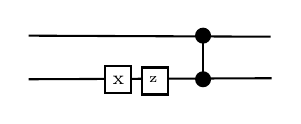
\begin{tikzpicture}[x=0.75pt,y=0.75pt,yscale=-1,xscale=1]
%uncomment if require: \path (0,300); %set diagram left start at 0, and has height of 300

%Straight Lines [id:da732813246379387] 
\draw    (99.83,109.67) -- (216.33,110.17) ;
%Straight Lines [id:da6605550224031504] 
\draw    (99.83,130.67) -- (216.83,130.17) ;
%Straight Lines [id:da2257066549092701] 
\draw    (183.83,109.67) -- (183.83,130.67) ;
\draw [shift={(183.83,130.67)}, rotate = 90] [color={rgb, 255:red, 0; green, 0; blue, 0 }  ][fill={rgb, 255:red, 0; green, 0; blue, 0 }  ][line width=0.75]      (0, 0) circle [x radius= 3.35, y radius= 3.35]   ;
\draw [shift={(183.83,109.67)}, rotate = 90] [color={rgb, 255:red, 0; green, 0; blue, 0 }  ][fill={rgb, 255:red, 0; green, 0; blue, 0 }  ][line width=0.75]      (0, 0) circle [x radius= 3.35, y radius= 3.35]   ;
%Shape: Rectangle [id:dp8096940990542667] 
\draw  [fill={rgb, 255:red, 255; green, 255; blue, 255 }  ,fill opacity=1 ] (136.8,124.5) -- (149.33,124.5) -- (149.33,137.5) -- (136.8,137.5) -- cycle ;
%Shape: Rectangle [id:dp33853823787750703] 
\draw  [fill={rgb, 255:red, 255; green, 255; blue, 255 }  ,fill opacity=1 ] (154.3,125) -- (166.83,125) -- (166.83,138) -- (154.3,138) -- cycle ;

% Text Node
\draw (138.8,127.5) node [anchor=north west][inner sep=0.75pt]  [font=\tiny] [align=left] {{\scriptsize x}};
% Text Node
\draw (156.3,128) node [anchor=north west][inner sep=0.75pt]  [font=\tiny] [align=left] {z};


\end{tikzpicture}

    \caption{Caption}
    \label{fig_APP:XZ-CZ}
\end{figure}

We start with \ref{fig_APP:XZ-CZ} which can be represented as $CZ(Z\otimes\mathbb{I})(X\otimes\mathbb{I})$ and then we just apply the identities we showed above:
\begin{align}
    CZ(Z\otimes\mathbb{I})(X\otimes\mathbb{I}) = (Z\otimes\mathbb{I})CZ(X\otimes\mathbb{I}) =
    (Z\otimes\mathbb{I})(X\otimes Z)CZ
\end{align}

This right-hand side is shown in \ref{fig_APP:CZ-XZ}. As we've shown for other gates, the qubit symmetry applies here as well so we can say that $CZ(\mathbb{I}\otimes Z)(\mathbb{I}\otimes X) = 
    (\mathbb{I}\otimes Z)(Z\otimes X)CZ$
\begin{figure}
    \centering

\tikzset{every picture/.style={line width=0.75pt}} %set default line width to 0.75pt        

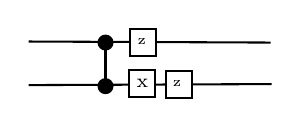
\begin{tikzpicture}[x=0.75pt,y=0.75pt,yscale=-1,xscale=1]
%uncomment if require: \path (0,300); %set diagram left start at 0, and has height of 300

%Straight Lines [id:da732813246379387] 
\draw    (99.83,109.67) -- (216.33,110.17) ;
%Straight Lines [id:da6605550224031504] 
\draw    (99.83,130.67) -- (216.83,130.17) ;
%Straight Lines [id:da2257066549092701] 
\draw    (136.83,110.17) -- (136.83,131.17) ;
\draw [shift={(136.83,131.17)}, rotate = 90] [color={rgb, 255:red, 0; green, 0; blue, 0 }  ][fill={rgb, 255:red, 0; green, 0; blue, 0 }  ][line width=0.75]      (0, 0) circle [x radius= 3.35, y radius= 3.35]   ;
\draw [shift={(136.83,110.17)}, rotate = 90] [color={rgb, 255:red, 0; green, 0; blue, 0 }  ][fill={rgb, 255:red, 0; green, 0; blue, 0 }  ][line width=0.75]      (0, 0) circle [x radius= 3.35, y radius= 3.35]   ;
%Shape: Rectangle [id:dp8096940990542667] 
\draw  [fill={rgb, 255:red, 255; green, 255; blue, 255 }  ,fill opacity=1 ] (148.3,123.5) -- (160.83,123.5) -- (160.83,136.5) -- (148.3,136.5) -- cycle ;
%Shape: Rectangle [id:dp33853823787750703] 
\draw  [fill={rgb, 255:red, 255; green, 255; blue, 255 }  ,fill opacity=1 ] (165.8,124) -- (178.33,124) -- (178.33,137) -- (165.8,137) -- cycle ;
%Shape: Rectangle [id:dp7489575253195708] 
\draw  [fill={rgb, 255:red, 255; green, 255; blue, 255 }  ,fill opacity=1 ] (148.8,103.5) -- (161.33,103.5) -- (161.33,116.5) -- (148.8,116.5) -- cycle ;

% Text Node
\draw (150.3,126.5) node [anchor=north west][inner sep=0.75pt]  [font=\tiny] [align=left] {{\scriptsize x}};
% Text Node
\draw (167.8,127) node [anchor=north west][inner sep=0.75pt]  [font=\tiny] [align=left] {z};
% Text Node
\draw (150.8,106.5) node [anchor=north west][inner sep=0.75pt]  [font=\tiny] [align=left] {z};


\end{tikzpicture}

    \caption{Caption}
    \label{fig_APP:CZ-XZ}
\end{figure}

\subsubsection{How CZ commutes with 2 X gates}
Here we'll look at how the CZ gate commutes with two X gates applied across 2 qubits. This looks like \ref{fig_APP:XX-CZ}. The trick to finding the commutation relation here revolves around splitting up the tensor product. We start with $CZ(X\otimes X)$):
\begin{equation}
    CZ(X\otimes X) = CZ(X\otimes \mathbb{I})(\mathbb{I}\otimes X)
\end{equation}
and then just like before we commute CZ through the equation on the right-hand side:
\begin{align}
    CZ(X\otimes X) &=  CZ(X\otimes \mathbb{I})(\mathbb{I}\otimes X)
    \\ & = (X\otimes Z)CZ(\mathbb{I}\otimes X)
    \\ & = (X\otimes Z)(Z\otimes X)CZ
\end{align}


\begin{figure}
    \centering
\tikzset{every picture/.style={line width=0.75pt}} %set default line width to 0.75pt        

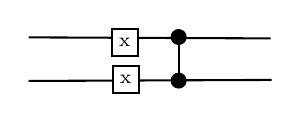
\begin{tikzpicture}[x=0.75pt,y=0.75pt,yscale=-1,xscale=1]
%uncomment if require: \path (0,300); %set diagram left start at 0, and has height of 300

%Straight Lines [id:da732813246379387] 
\draw    (99.83,109.67) -- (216.33,110.17) ;
%Straight Lines [id:da6605550224031504] 
\draw    (99.83,130.67) -- (216.83,130.17) ;
%Straight Lines [id:da2257066549092701] 
\draw    (172.07,109.5) -- (172.07,130.5) ;
\draw [shift={(172.07,130.5)}, rotate = 90] [color={rgb, 255:red, 0; green, 0; blue, 0 }  ][fill={rgb, 255:red, 0; green, 0; blue, 0 }  ][line width=0.75]      (0, 0) circle [x radius= 3.35, y radius= 3.35]   ;
\draw [shift={(172.07,109.5)}, rotate = 90] [color={rgb, 255:red, 0; green, 0; blue, 0 }  ][fill={rgb, 255:red, 0; green, 0; blue, 0 }  ][line width=0.75]      (0, 0) circle [x radius= 3.35, y radius= 3.35]   ;
%Shape: Rectangle [id:dp8096940990542667] 
\draw  [fill={rgb, 255:red, 255; green, 255; blue, 255 }  ,fill opacity=1 ] (140.3,123.5) -- (152.83,123.5) -- (152.83,136.5) -- (140.3,136.5) -- cycle ;
%Shape: Rectangle [id:dp4624452996610504] 
\draw  [fill={rgb, 255:red, 255; green, 255; blue, 255 }  ,fill opacity=1 ] (139.8,105.5) -- (152.33,105.5) -- (152.33,118.5) -- (139.8,118.5) -- cycle ;

% Text Node
\draw (142.3,126.5) node [anchor=north west][inner sep=0.75pt]  [font=\tiny] [align=left] {{\scriptsize x}};
% Text Node
\draw (141.8,108.5) node [anchor=north west][inner sep=0.75pt]  [font=\tiny] [align=left] {{\scriptsize x}};

\end{tikzpicture}
    \caption{Caption}
    \label{fig_APP:XX-CZ}
\end{figure}

The right-hand side is shown in \ref{fig_APP:CZ - ZX,xZ}.

\begin{figure}
    \centering
\tikzset{every picture/.style={line width=0.75pt}} %set default line width to 0.75pt        

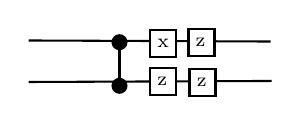
\begin{tikzpicture}[x=0.75pt,y=0.75pt,yscale=-1,xscale=1]
%uncomment if require: \path (0,300); %set diagram left start at 0, and has height of 300

%Straight Lines [id:da732813246379387] 
\draw    (99.83,110.67) -- (216.33,111.17) ;
%Straight Lines [id:da6605550224031504] 
\draw    (99.83,130.67) -- (216.83,130.17) ;
%Straight Lines [id:da2257066549092701] 
\draw    (143.57,111.5) -- (143.57,132.5) ;
\draw [shift={(143.57,132.5)}, rotate = 90] [color={rgb, 255:red, 0; green, 0; blue, 0 }  ][fill={rgb, 255:red, 0; green, 0; blue, 0 }  ][line width=0.75]      (0, 0) circle [x radius= 3.35, y radius= 3.35]   ;
\draw [shift={(143.57,111.5)}, rotate = 90] [color={rgb, 255:red, 0; green, 0; blue, 0 }  ][fill={rgb, 255:red, 0; green, 0; blue, 0 }  ][line width=0.75]      (0, 0) circle [x radius= 3.35, y radius= 3.35]   ;
%Shape: Rectangle [id:dp8096940990542667] 
\draw  [fill={rgb, 255:red, 255; green, 255; blue, 255 }  ,fill opacity=1 ] (177.3,124.5) -- (189.83,124.5) -- (189.83,137.5) -- (177.3,137.5) -- cycle ;
%Shape: Rectangle [id:dp4624452996610504] 
\draw  [fill={rgb, 255:red, 255; green, 255; blue, 255 }  ,fill opacity=1 ] (158.3,105.5) -- (170.83,105.5) -- (170.83,118.5) -- (158.3,118.5) -- cycle ;
%Shape: Rectangle [id:dp21808645132641424] 
\draw  [fill={rgb, 255:red, 255; green, 255; blue, 255 }  ,fill opacity=1 ] (158.3,124) -- (170.83,124) -- (170.83,137) -- (158.3,137) -- cycle ;
%Shape: Rectangle [id:dp008241843524475545] 
\draw  [fill={rgb, 255:red, 255; green, 255; blue, 255 }  ,fill opacity=1 ] (176.8,105) -- (189.33,105) -- (189.33,118) -- (176.8,118) -- cycle ;

% Text Node
\draw (179.3,127.5) node [anchor=north west][inner sep=0.75pt]  [font=\tiny] [align=left] {{\scriptsize z}};
% Text Node
\draw (160.3,108.5) node [anchor=north west][inner sep=0.75pt]  [font=\tiny] [align=left] {{\scriptsize x}};
% Text Node
\draw (160.3,127) node [anchor=north west][inner sep=0.75pt]  [font=\tiny] [align=left] {{\scriptsize z}};
% Text Node
\draw (178.8,108) node [anchor=north west][inner sep=0.75pt]  [font=\tiny] [align=left] {{\scriptsize z}};


\end{tikzpicture}
    \caption{Caption}
    \label{fig_APP:CZ - ZX,xZ}
\end{figure}

\subsubsection{How CZ commutes with 2 XZ gate combinations}
We're going to skip all the other kinds of combinations that can be done with X and Z gates commuting with CZ and focus on how CZ commutes through an X and Z gate applied to both qubits. We start with $CZ(X\otimes X)(Z\otimes Z)$:
\begin{align}
    CZ(X\otimes X)(Z\otimes Z) & = (X\otimes Z)(Z\otimes X)CZ(Z\otimes Z)
    \\ & = (X\otimes Z)(Z\otimes X)(Z\otimes Z)CZ
\end{align}
We can then simplify this using the fact that $X \cdot X \equiv \mathbb{I}$ and $Z \cdot Z \equiv \mathbb{I}$:

\begin{align}
    CZ(X\otimes X)(Z\otimes Z) & = (X\otimes Z)(Z\otimes X)(Z\otimes Z)CZ
    \\ & = (X\otimes Z)(Z\otimes\mathbb{I})(\mathbb{I}\otimes X)(Z\otimes\mathbb{I})(\mathbb{I}\otimes Z)CZ
    \\ & = (X\otimes Z)(\mathbb{I}\otimes X)(Z\otimes\mathbb{I})(Z\otimes\mathbb{I})(\mathbb{I}\otimes Z)CZ \label{qubit order swap}
    \\ & = (X\otimes Z)(\mathbb{I}\otimes X)(\mathbb{I}\otimes Z)CZ
\end{align}
where in \ref{qubit order swap} we use the fact that $(Z\otimes\mathbb{I})$ commutes with $(\mathbb{I}\otimes X)$ since these are single qubit gate operators acting on different qubits.
\par
What makes this result interesting is that because the left-hand side of the above equation is symmetric, our result is equal to its qubit symmetric pair. Meaning that:
\begin{equation}
     CZ(X\otimes X)(Z\otimes Z) = (X\otimes Z)(\mathbb{I}\otimes X)(\mathbb{I}\otimes Z)CZ = (Z\otimes X)(X\otimes \mathbb{I})(Z\otimes \mathbb{I})CZ
\end{equation}